Illustrated in \cref{fig:five-polys} is the bicentric family along with its two limiting-pedals and its two polar images (elliptic and hyperbolic billiards), each with respect to a limiting point. While N-periodics in the elliptic billiard conserves perimeter, it turns out their hyperbolic versions conserve their {\em signed} perimeter, i.e., the length of segments on where both (just one) coordinates change sign are counted as negative (resp. positive).

Indeed \cref{fig:bicentric-diagram} illustrates that the bicentric family is a kind of ``hub'' from which four equiperimeter (and of constant cosine sum) derived polygon families can be obtained. Bicentrics themselves have variable perimeter.

\begin{figure}
    \centering
    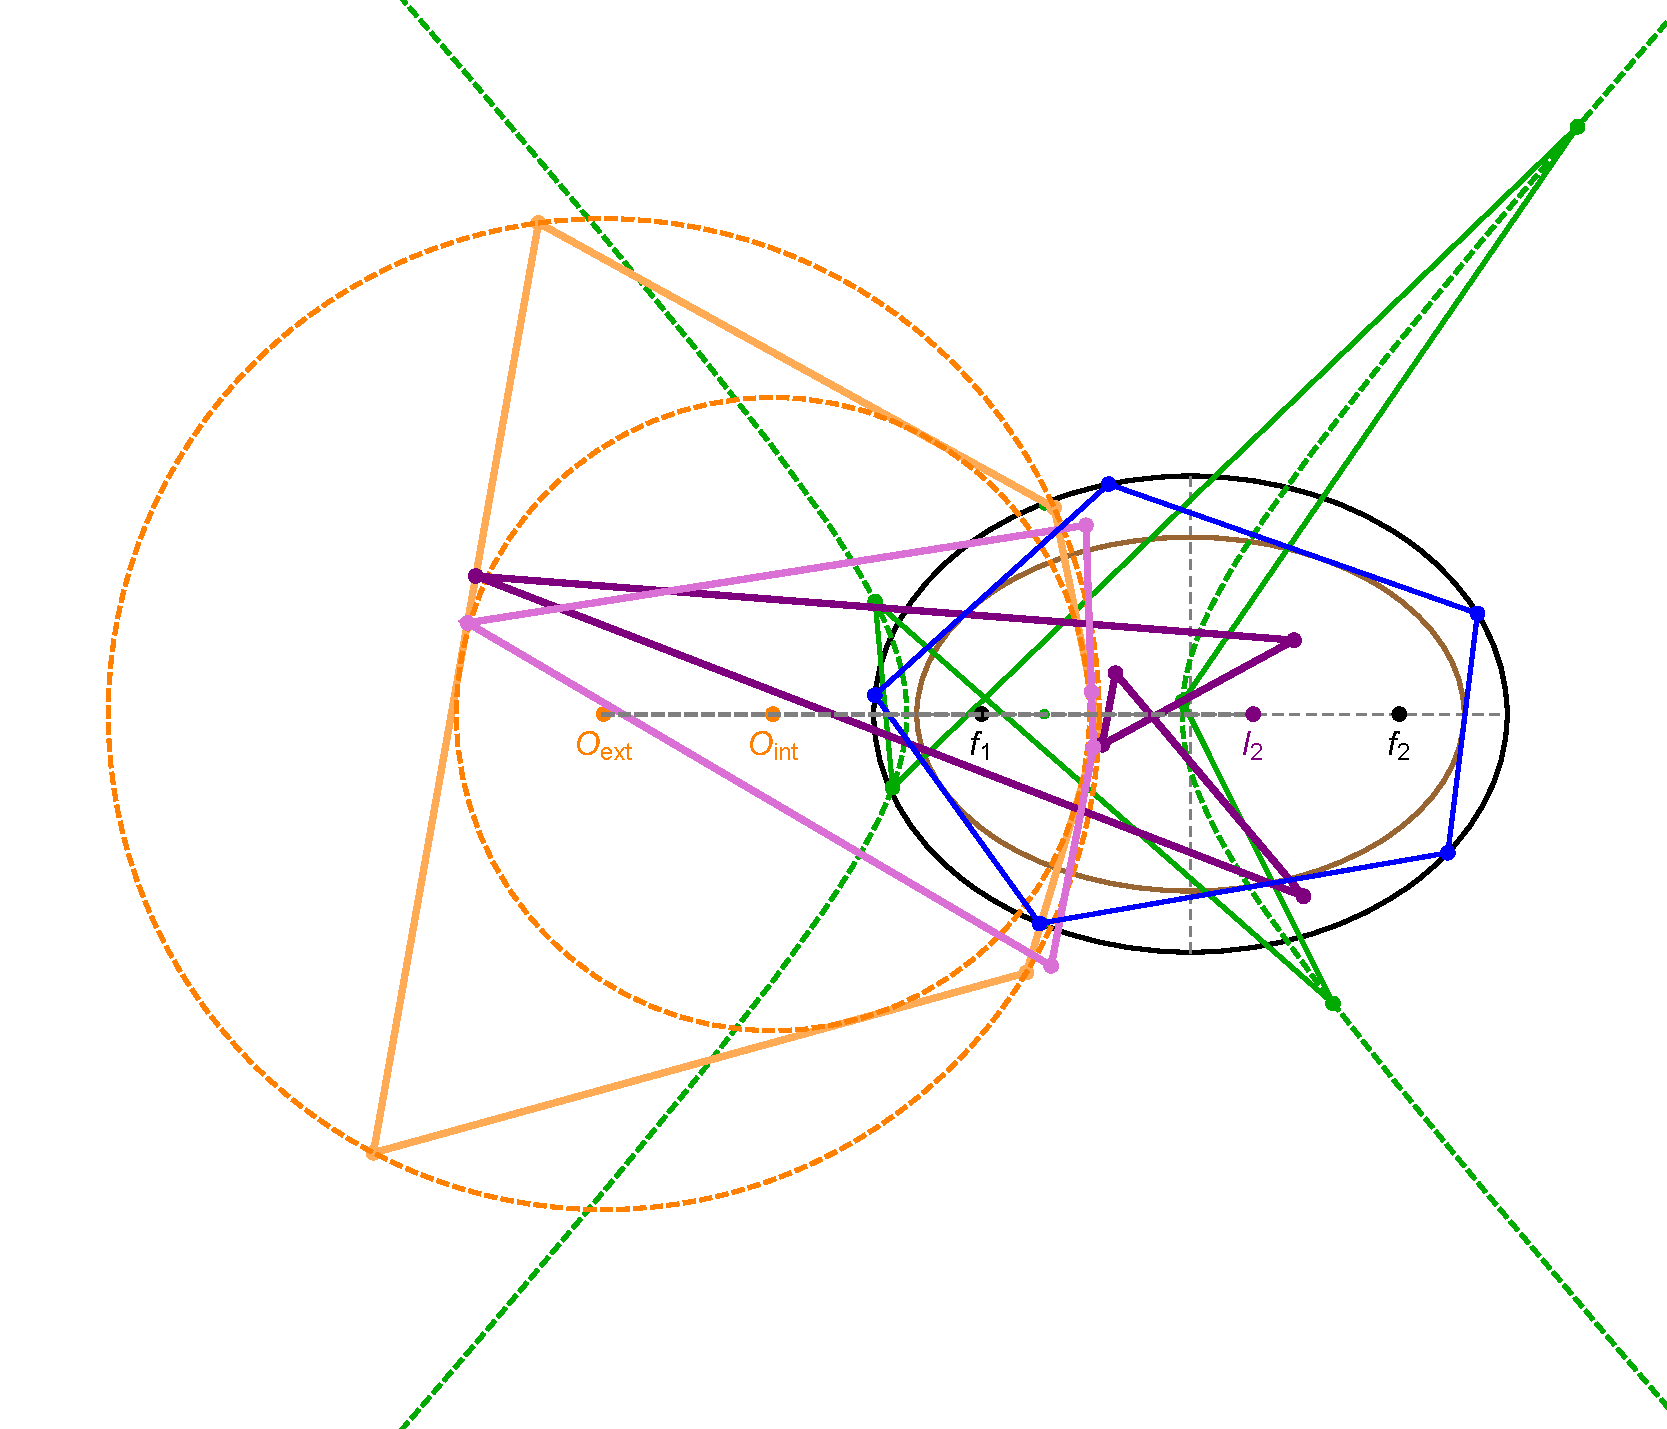
\includegraphics[width=\textwidth]{pics/0130_five_polys.pdf}
    \caption{The bicentric family (solid orange), its two polar images: the elliptic billiard (blue) and the hyperbolic biliard (green), and the two limiting pedal polygons (pink and purple). All but the bicentrics are equiperimetric. All conserve their sum of cosines.}
    \label{fig:five-polys}
\end{figure}


\begin{figure}
    \centering
    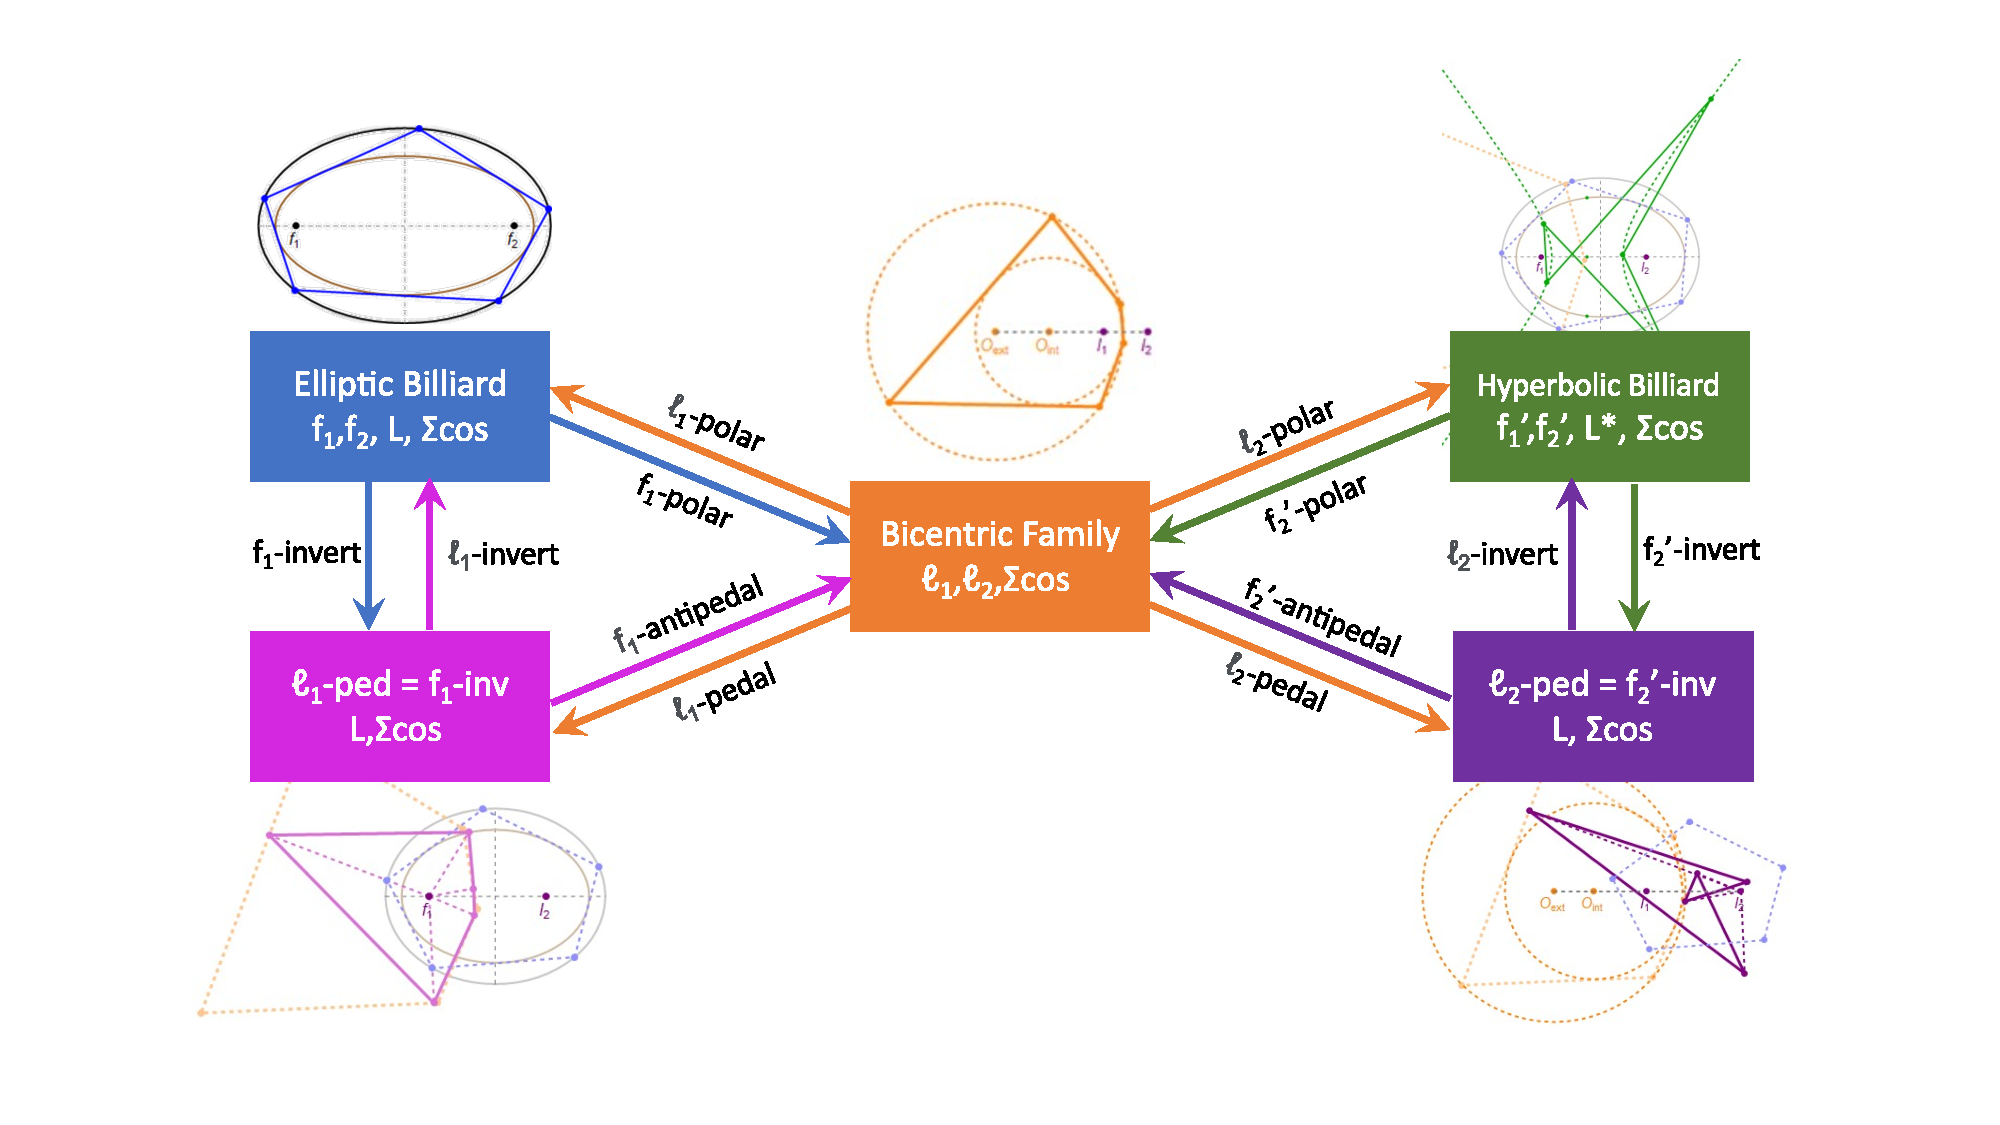
\includegraphics[trim=100 50 100 50,clip,width=\textwidth]{pics/0140_bicentric_diagram.pdf}
    \caption{The bicentric family (orange, center) is the hub from which four polygon families can be derived: the (i) elliptic (resp. (ii) hyperbolic) billiard with foci $f_1=\ell_1,f_2$ (resp. $f_1'$ and $f_2'=\ell_2$) is the bicentric polar image with respect to $\ell_1$ (resp. $\ell_2$); (iii) the first (resp. second) pedal is obtained with respect to $\ell_1$ (resp. $\ell_2$). These are the inversive image of the elliptic and hyperbolic billiards with respect to $l_1=f_1$ or $l_2=f_2'$, respectively. With the exception of the bicentrics, all 4 derived families conserve perimeter $L$ (in the case of the hyperbolic billiard it is the {\em signed} perimeter $L^*$ which is conserved. All 5 families conserve sum of cosines, except for $N=4$ $\ell_1$-pedals.}
    \label{fig:bicentric-diagram}
\end{figure}